Việc triển khai cơ sở dữ liệu của hệ thống được thực hiện trên nền tảng Neon.tech.
Sau khi hoàn tất việc tạo tài khoản hoặc đăng nhập vào Neon.tech, chúng ta sẽ tạo một Database ở trên nền tảng này:
\begin{figure}[H]
    \centering
    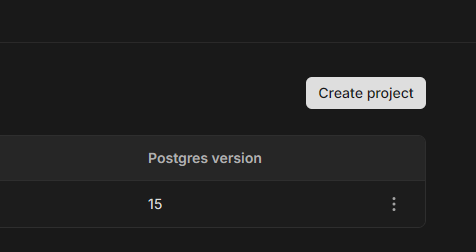
\includegraphics[width=0.5\linewidth]{Content/Hiện thực hệ thống/images/createProjectDB.png}
    \vspace{0.5cm}
    \caption{Giao diện tạo Database trên Neon.tech}
    \label{fig:Tạo Database}
\end{figure}
Sau đó, ta sẽ điều chỉnh một số thông tin về database, chẳng hạn như tên, server lưu trữ:
\begin{figure}[H]
    \centering
    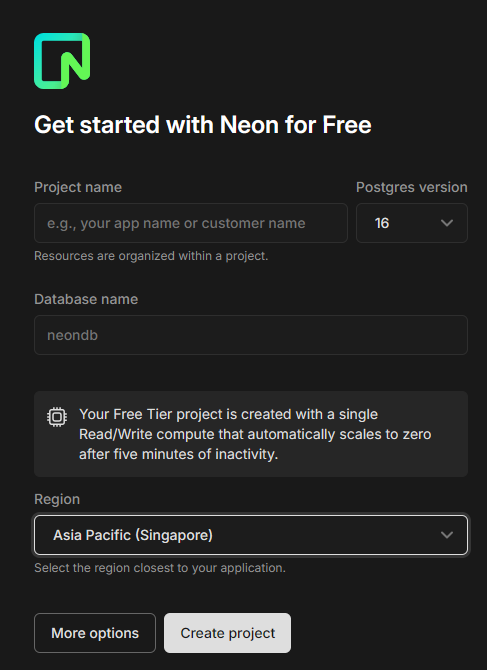
\includegraphics[width=0.5\linewidth]{Content/Hiện thực hệ thống/images/projectDBinfo.png}
    \vspace{0.5cm}
    \caption{Điều chỉnh thông tin Database trên Neon.tech}
    \label{fig:Điều chỉnh thông tin Database}
\end{figure}
Cuối cùng, việc tạo database đã hoàn tất. Neon.tech sẽ tạo ra đường dẫn để ta có thể kết nối tới database này. Ngoài ra,
Neon.tech còn hỗ trợ viết câu lệnh truy vấn, giúp ta có thể thao tác với database một cách dễ dàng.
\begin{figure}[H]
    \centering
    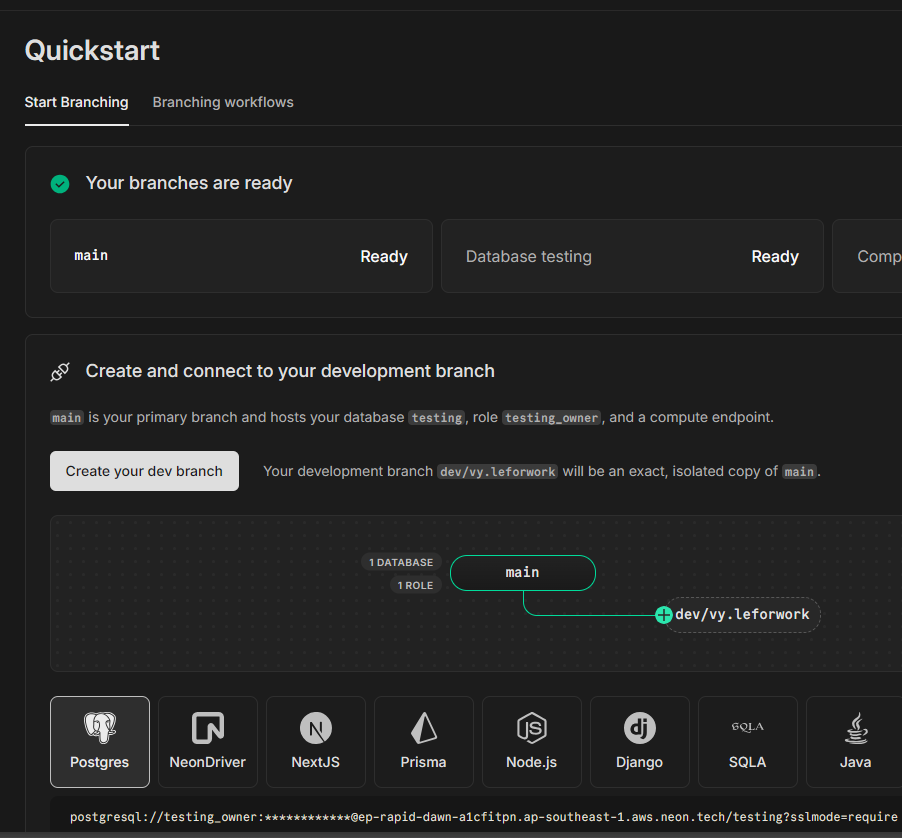
\includegraphics[width=0.5\linewidth]{Content/Hiện thực hệ thống/images/finishDBcreate.png}
    \vspace{0.5cm}
    \caption{Khởi tạo Database thành công}
    \label{fig:Khởi tạo Database thành công}
\end{figure}